\chapter{Additional Results}
\label{chapter:appendix-results}

This appendix contains additional results of our experiments which complement chapter \ref{chapter:results}.

% EX01 - Pebbles
\begin{figure}[]
    \centering    
    \begin{subfigure}{\textwidth}
        \centering
        \begin{subfigure}{0.24\textwidth}
            \centering
            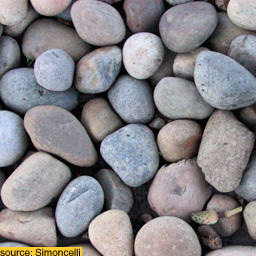
\includegraphics[width=\textwidth]{images/04-experiment01/pebbles/target.jpg}
            \caption*{}
        \end{subfigure}
        \hfill
        \begin{subfigure}{0.24\textwidth}
            \centering
            
\includegraphics[width=\textwidth]{images/04-experiment01/pebbles/white_bg.jpg}
            \caption*{}
        \end{subfigure}
        \hfill
        \begin{subfigure}{0.24\textwidth}
            \centering
            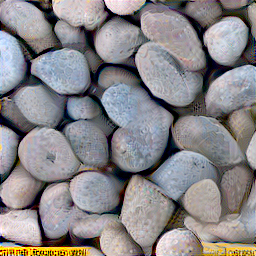
\includegraphics[width=\textwidth]{images/04-experiment01/pebbles/1000/white_im.jpg}
            \caption*{}
        \end{subfigure}
        \hfill
        \begin{subfigure}{0.24\textwidth}
            \centering
            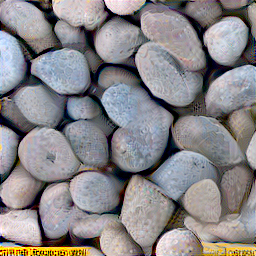
\includegraphics[width=\textwidth]{images/04-experiment01/pebbles/1000/white_proj.jpg}
            \caption*{}
        \end{subfigure}

        \begin{subfigure}{0.24\textwidth}
            \centering
            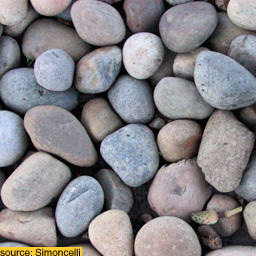
\includegraphics[width=\textwidth]{images/04-experiment01/pebbles/target.jpg}
            \caption*{}
        \end{subfigure}
        \hfill
        \begin{subfigure}{0.24\textwidth}
            \centering
            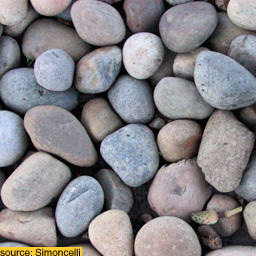
\includegraphics[width=\textwidth]{images/04-experiment01/pebbles/pebbles_bg.jpg}
            \caption*{}
        \end{subfigure}
        \hfill
        \begin{subfigure}{0.24\textwidth}
            \centering
            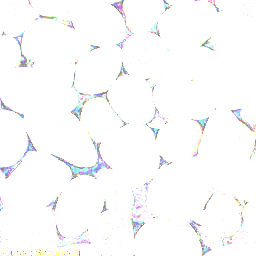
\includegraphics[width=\textwidth]{images/04-experiment01/pebbles/1000/pebbles_im.jpg}
            \caption*{}
        \end{subfigure}
        \hfill
        \begin{subfigure}{0.24\textwidth}
            \centering
            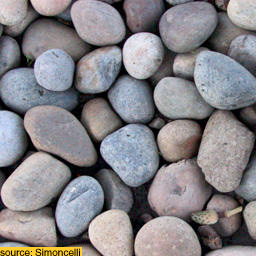
\includegraphics[width=\textwidth]{images/04-experiment01/pebbles/1000/pebbles_proj.jpg}
            \caption*{}
        \end{subfigure}

        \begin{subfigure}{0.24\textwidth}
            \centering
            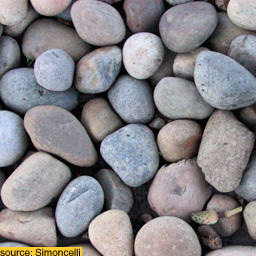
\includegraphics[width=\textwidth]{images/04-experiment01/pebbles/target.jpg}
            \caption*{}
        \end{subfigure}
        \hfill
        \begin{subfigure}{0.24\textwidth}
            \centering
            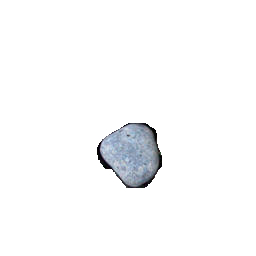
\includegraphics[width=\textwidth]{images/04-experiment01/pebbles/one_bg.jpg}
            \caption*{}
        \end{subfigure}
        \hfill
        \begin{subfigure}{0.24\textwidth}
            \centering
            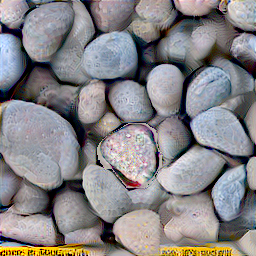
\includegraphics[width=\textwidth]{images/04-experiment01/pebbles/1000/one_im.jpg}
            \caption*{}
        \end{subfigure}
        \hfill
        \begin{subfigure}{0.24\textwidth}
            \centering
            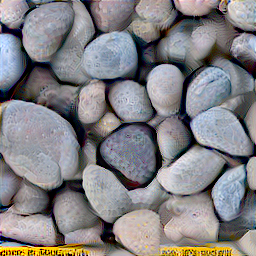
\includegraphics[width=\textwidth]{images/04-experiment01/pebbles/1000/one_proj.jpg}
            \caption*{}
        \end{subfigure}

        \begin{subfigure}{0.24\textwidth}
            \centering
            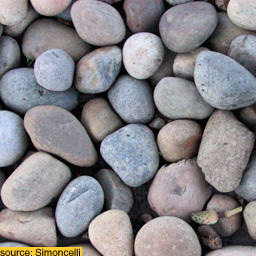
\includegraphics[width=\textwidth]{images/04-experiment01/pebbles/target.jpg}
            \caption*{}
        \end{subfigure}
        \hfill
        \begin{subfigure}{0.24\textwidth}
            \centering
            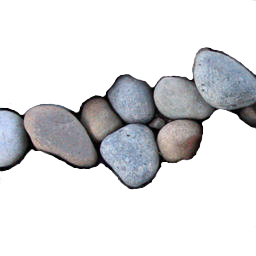
\includegraphics[width=\textwidth]{images/04-experiment01/pebbles/some_bg.jpg}
            \caption*{}
        \end{subfigure}
        \hfill
        \begin{subfigure}{0.24\textwidth}
            \centering
            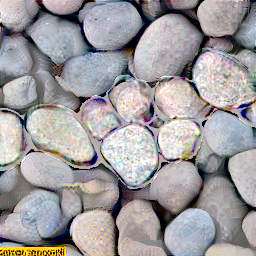
\includegraphics[width=\textwidth]{images/04-experiment01/pebbles/1000/some_im.jpg}
            \caption*{}
        \end{subfigure}
        \hfill
        \begin{subfigure}{0.24\textwidth}
            \centering
            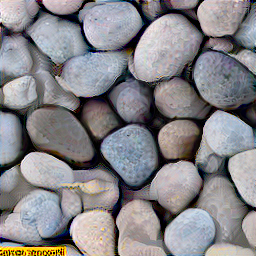
\includegraphics[width=\textwidth]{images/04-experiment01/pebbles/1000/some_proj.jpg}
            \caption*{}
        \end{subfigure}
        
        \begin{subfigure}{0.24\textwidth}
            \centering
            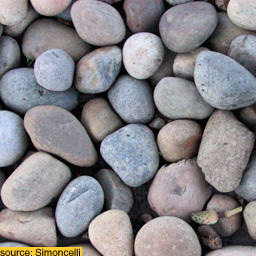
\includegraphics[width=\textwidth]{images/04-experiment01/pebbles/target.jpg}
            \caption*{Input}
        \end{subfigure}
        \hfill
        \begin{subfigure}{0.24\textwidth}
            \centering
            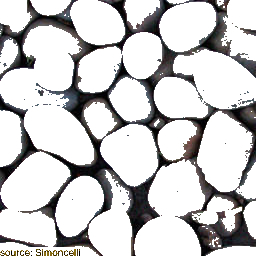
\includegraphics[width=\textwidth]{images/04-experiment01/pebbles/threshold_bg.jpg}
            \caption*{Background}
        \end{subfigure}
        \hfill
        \begin{subfigure}{0.24\textwidth}
            \centering
            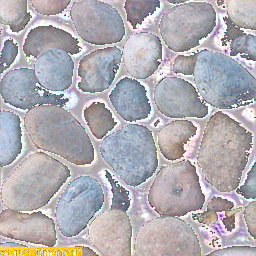
\includegraphics[width=\textwidth]{images/04-experiment01/pebbles/1000/threshold_im.jpg}
            \caption*{Compensation}
        \end{subfigure}
        \hfill
        \begin{subfigure}{0.24\textwidth}
            \centering
            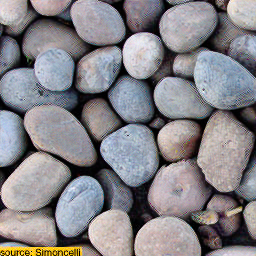
\includegraphics[width=\textwidth]{images/04-experiment01/pebbles/1000/threshold_proj.jpg}
            \caption*{Camera image}
        \end{subfigure}
    \end{subfigure}
    \caption{These results complement section \ref{section:results-experiments-01}. Texture source: \citet{Gatys2015}}
    \label{fig:ex01-complete-pebbles-1000steps}
\end{figure}

% EX01 - Flowers
\begin{figure}[]
    \centering    
    \begin{subfigure}{\textwidth}
        \centering
        \begin{subfigure}{0.24\textwidth}
            \centering
            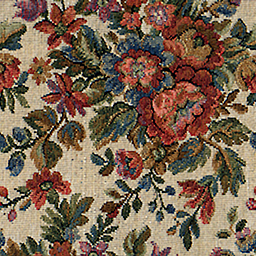
\includegraphics[width=\textwidth]{images/04-experiment01/flowers/target.jpg}
            \caption*{}
        \end{subfigure}
        \hfill
        \begin{subfigure}{0.24\textwidth}
            \centering
            
\includegraphics[width=\textwidth]{images/04-experiment01/flowers/white_bg.jpg}
            \caption*{}
        \end{subfigure}
        \hfill
        \begin{subfigure}{0.24\textwidth}
            \centering
            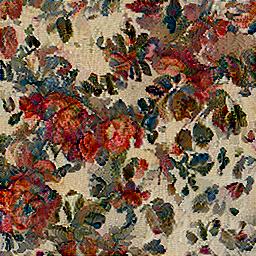
\includegraphics[width=\textwidth]{images/04-experiment01/flowers/1000/white_im.jpg}
            \caption*{}
        \end{subfigure}
        \hfill
        \begin{subfigure}{0.24\textwidth}
            \centering
            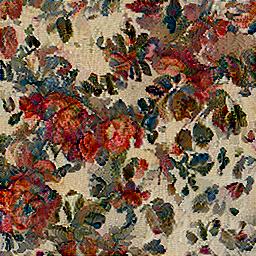
\includegraphics[width=\textwidth]{images/04-experiment01/flowers/1000/white_proj.jpg}
            \caption*{}
        \end{subfigure}

        \begin{subfigure}{0.24\textwidth}
            \centering
            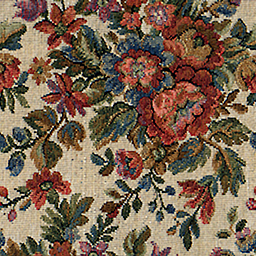
\includegraphics[width=\textwidth]{images/04-experiment01/flowers/target.jpg}
            \caption*{}
        \end{subfigure}
        \hfill
        \begin{subfigure}{0.24\textwidth}
            \centering
            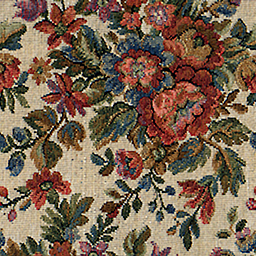
\includegraphics[width=\textwidth]{images/04-experiment01/flowers/flowers_bg.jpg}
            \caption*{}
        \end{subfigure}
        \hfill
        \begin{subfigure}{0.24\textwidth}
            \centering
            
\includegraphics[width=\textwidth]{images/04-experiment01/flowers/1000/flowers_im.jpg}
            \caption*{}
        \end{subfigure}
        \hfill
        \begin{subfigure}{0.24\textwidth}
            \centering
            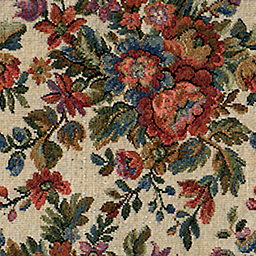
\includegraphics[width=\textwidth]{images/04-experiment01/flowers/1000/flowers_proj.jpg}
            \caption*{}
        \end{subfigure}

        \begin{subfigure}{0.24\textwidth}
            \centering
            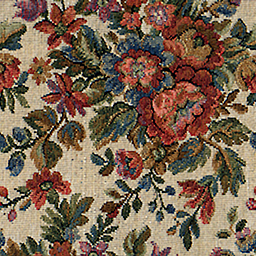
\includegraphics[width=\textwidth]{images/04-experiment01/flowers/target.jpg}
            \caption*{}
        \end{subfigure}
        \hfill
        \begin{subfigure}{0.24\textwidth}
            \centering
            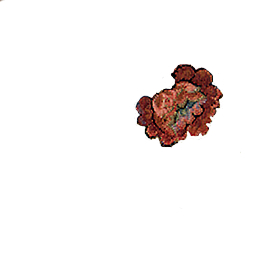
\includegraphics[width=\textwidth]{images/04-experiment01/flowers/one_bg.jpg}
            \caption*{}
        \end{subfigure}
        \hfill
        \begin{subfigure}{0.24\textwidth}
            \centering
            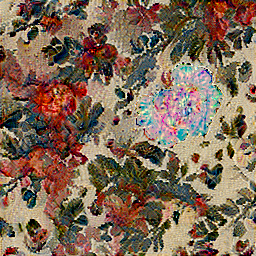
\includegraphics[width=\textwidth]{images/04-experiment01/flowers/1000/one_im.jpg}
            \caption*{}
        \end{subfigure}
        \hfill
        \begin{subfigure}{0.24\textwidth}
            \centering
            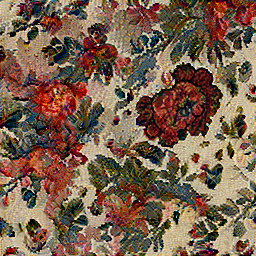
\includegraphics[width=\textwidth]{images/04-experiment01/flowers/1000/one_proj.jpg}
            \caption*{}
        \end{subfigure}

        \begin{subfigure}{0.24\textwidth}
            \centering
            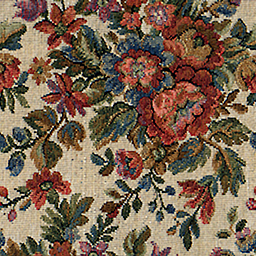
\includegraphics[width=\textwidth]{images/04-experiment01/flowers/target.jpg}
            \caption*{}
        \end{subfigure}
        \hfill
        \begin{subfigure}{0.24\textwidth}
            \centering
            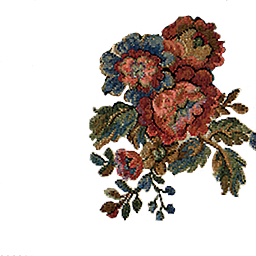
\includegraphics[width=\textwidth]{images/04-experiment01/flowers/some_bg.jpg}
            \caption*{}
        \end{subfigure}
        \hfill
        \begin{subfigure}{0.24\textwidth}
            \centering
            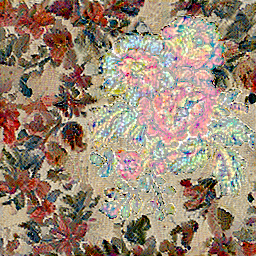
\includegraphics[width=\textwidth]{images/04-experiment01/flowers/1000/some_im.jpg}
            \caption*{}
        \end{subfigure}
        \hfill
        \begin{subfigure}{0.24\textwidth}
            \centering
            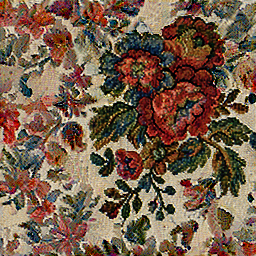
\includegraphics[width=\textwidth]{images/04-experiment01/flowers/1000/some_proj.jpg}
            \caption*{}
        \end{subfigure}
        
        \begin{subfigure}{0.24\textwidth}
            \centering
            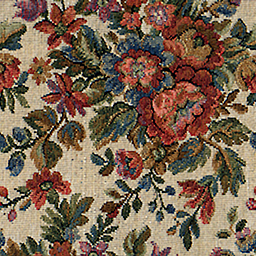
\includegraphics[width=\textwidth]{images/04-experiment01/flowers/target.jpg}
            \caption*{Input}
        \end{subfigure}
        \hfill
        \begin{subfigure}{0.24\textwidth}
            \centering
            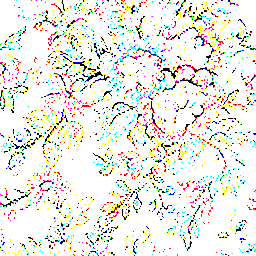
\includegraphics[width=\textwidth]{images/04-experiment01/flowers/threshold_bg.jpg}
            \caption*{Background}
        \end{subfigure}
        \hfill
        \begin{subfigure}{0.24\textwidth}
            \centering
            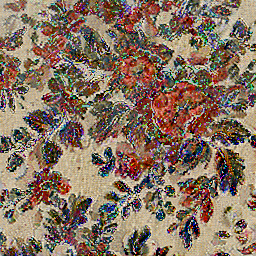
\includegraphics[width=\textwidth]{images/04-experiment01/flowers/1000/threshold_im.jpg}
            \caption*{Compensation}
        \end{subfigure}
        \hfill
        \begin{subfigure}{0.24\textwidth}
            \centering
            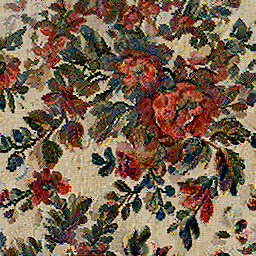
\includegraphics[width=\textwidth]{images/04-experiment01/flowers/1000/threshold_proj.jpg}
            \caption*{Camera image}
        \end{subfigure}
    \end{subfigure}
    \caption{These results complement section \ref{section:results-experiments-01}. Texture source: \citet{Pixar128}}
    \label{fig:ex01-complete-flowers-1000steps}
\end{figure}

% EX02 - Human - Marble, wood
\begin{figure}[]
    \centering    
    \begin{subfigure}{\textwidth}
        \centering
        \begin{subfigure}{0.24\textwidth}
            \centering
            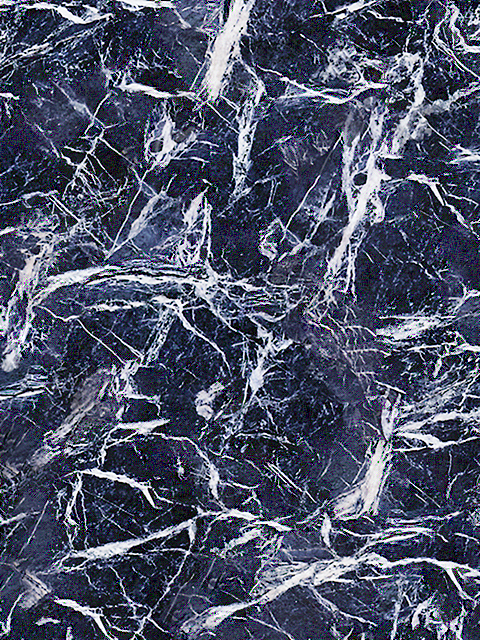
\includegraphics[width=\textwidth]{images/04-experiment02/human/marble/target.jpg}
            \caption*{Input}
        \end{subfigure}
        \hfill
        \begin{subfigure}{0.24\textwidth}
            \centering
            
\includegraphics[width=\textwidth]{images/04-experiment02/human/bg.jpg}
            \caption*{Background}
        \end{subfigure}
        \hfill
        \begin{subfigure}{0.24\textwidth}
            \centering
            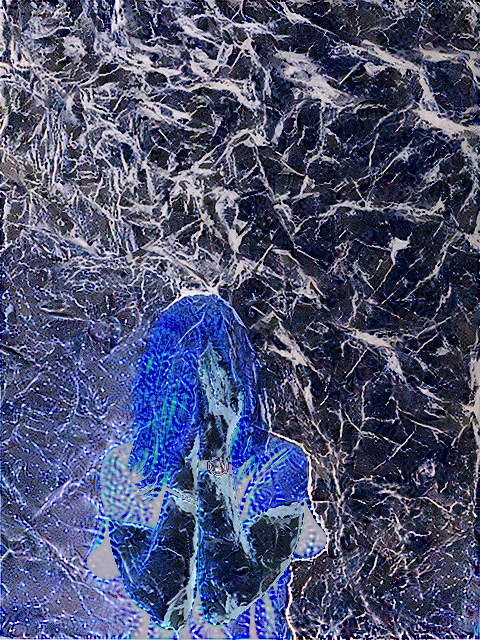
\includegraphics[width=\textwidth]{images/04-experiment02/human/marble/gatys_im.jpg}
            \caption*{Gatys comp.}
        \end{subfigure}
        \hfill
        \begin{subfigure}{0.24\textwidth}
            \centering
            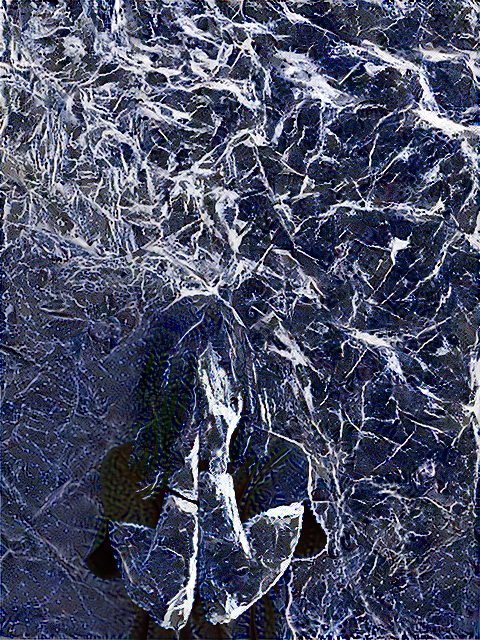
\includegraphics[width=\textwidth]{images/04-experiment02/human/marble/gatys_proj.jpg}
            \caption*{Gatys camera}
        \end{subfigure}
        
        \begin{subfigure}{0.24\textwidth}
            \centering
            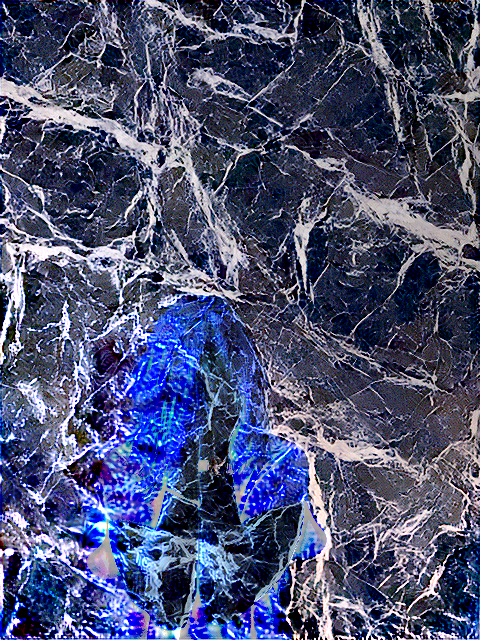
\includegraphics[width=\textwidth]{images/04-experiment02/human/marble/improved_im.jpg}
            \caption*{Improved comp.}
        \end{subfigure}
        \hfill
        \begin{subfigure}{0.24\textwidth}
            \centering
            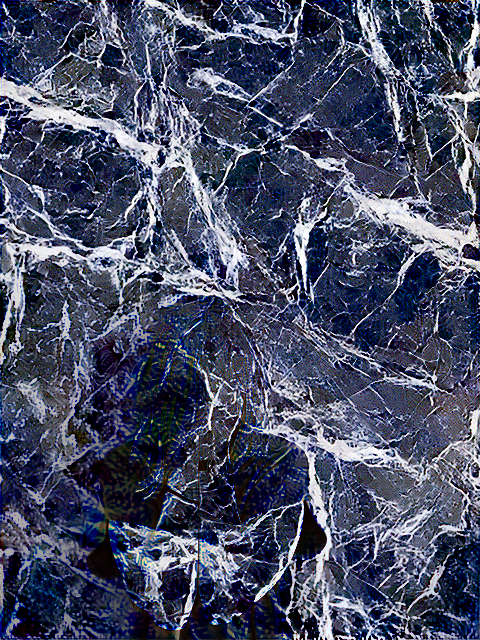
\includegraphics[width=\textwidth]{images/04-experiment02/human/marble/improved_proj.jpg}
            \caption*{Improved cam.}
        \end{subfigure}
        \hfill
        \begin{subfigure}{0.24\textwidth}
            \centering
            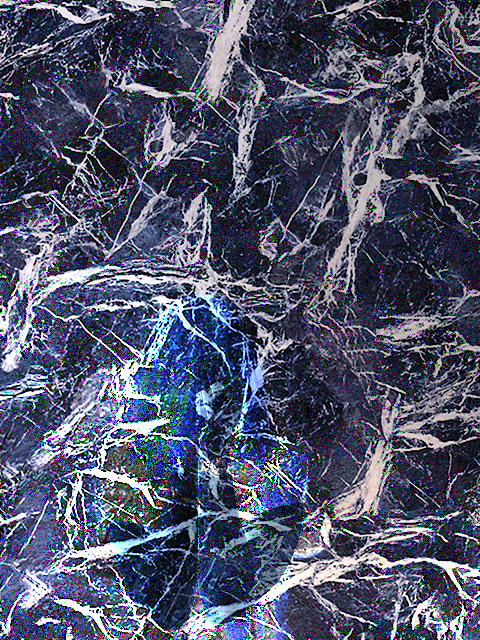
\includegraphics[width=\textwidth]{images/04-experiment02/human/marble/pixel_im.jpg}
            \caption*{Pixel comp.}
        \end{subfigure}
        \hfill
        \begin{subfigure}{0.24\textwidth}
            \centering
            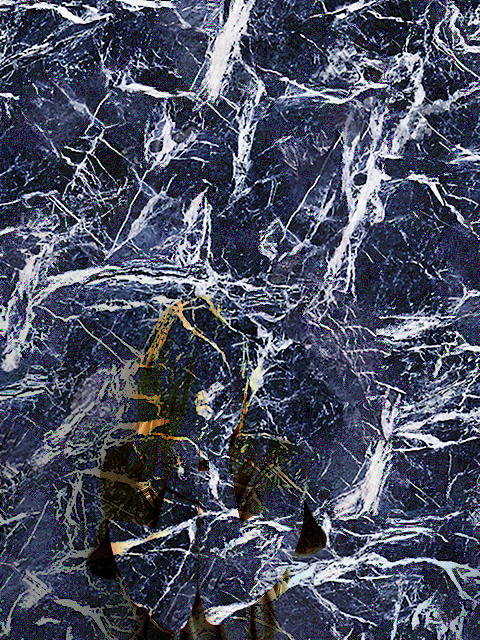
\includegraphics[width=\textwidth]{images/04-experiment02/human/marble/pixel_proj.jpg}
            \caption*{Pixel camera}
        \end{subfigure}
    \end{subfigure}

    \begin{subfigure}{\textwidth}
        \centering
        \begin{subfigure}{0.24\textwidth}
            \centering
            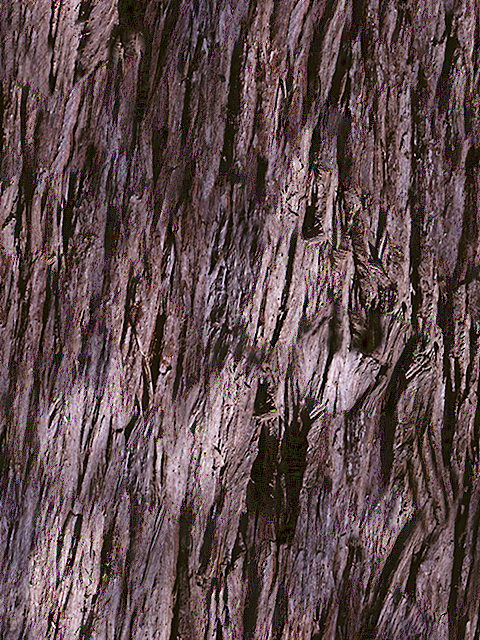
\includegraphics[width=\textwidth]{images/04-experiment02/human/wood/target.jpg}
            \caption*{Input}
        \end{subfigure}
        \hfill
        \begin{subfigure}{0.24\textwidth}
            \centering
            
\includegraphics[width=\textwidth]{images/04-experiment02/human/bg.jpg}
            \caption*{Background}
        \end{subfigure}
        \hfill
        \begin{subfigure}{0.24\textwidth}
            \centering
            \includegraphics[width=\textwidth]{images/04-experiment02/human/wood/gatys_im.jpg}
            \caption*{Gatys comp.}
        \end{subfigure}
        \hfill
        \begin{subfigure}{0.24\textwidth}
            \centering
            \includegraphics[width=\textwidth]{images/04-experiment02/human/wood/gatys_proj.jpg}
            \caption*{Gatys camera}
        \end{subfigure}
        
        \begin{subfigure}{0.24\textwidth}
            \centering
            \includegraphics[width=\textwidth]{images/04-experiment02/human/wood/improved_im.jpg}
            \caption*{Improved comp.}
        \end{subfigure}
        \hfill
        \begin{subfigure}{0.24\textwidth}
            \centering
            \includegraphics[width=\textwidth]{images/04-experiment02/human/wood/improved_proj.jpg}
            \caption*{Improved cam.}
        \end{subfigure}
        \hfill
        \begin{subfigure}{0.24\textwidth}
            \centering
            \includegraphics[width=\textwidth]{images/04-experiment02/human/wood/pixel_im.jpg}
            \caption*{Pixel comp.}
        \end{subfigure}
        \hfill
        \begin{subfigure}{0.24\textwidth}
            \centering
            \includegraphics[width=\textwidth]{images/04-experiment02/human/wood/pixel_proj.jpg}
            \caption*{Pixel camera}
        \end{subfigure}
    \end{subfigure}
    \caption{These results complement section \ref{section:results-experiments-02}. Texture source: \citet{Pixar128}}
    \label{fig:ex02-complete-human-marble_wood}
\end{figure}

% EX02 - Human - Flowers, flowers2
\begin{figure}[]
    \centering    
    \begin{subfigure}{\textwidth}
        \centering
        \begin{subfigure}{0.24\textwidth}
            \centering
            \includegraphics[width=\textwidth]{images/04-experiment02/human/flowers/target.jpg}
            \caption*{Input}
        \end{subfigure}
        \hfill
        \begin{subfigure}{0.24\textwidth}
            \centering
            \includegraphics[width=\textwidth]{images/04-experiment02/human/bg.jpg}
            \caption*{Background}
        \end{subfigure}
        \hfill
        \begin{subfigure}{0.24\textwidth}
            \centering
            \includegraphics[width=\textwidth]{images/04-experiment02/human/flowers/gatys_im.jpg}
            \caption*{Gatys comp.}
        \end{subfigure}
        \hfill
        \begin{subfigure}{0.24\textwidth}
            \centering
            \includegraphics[width=\textwidth]{images/04-experiment02/human/flowers/gatys_proj.jpg}
            \caption*{Gatys camera}
        \end{subfigure}
        
        \begin{subfigure}{0.24\textwidth}
            \centering
            \includegraphics[width=\textwidth]{images/04-experiment02/human/flowers/improved_im.jpg}
            \caption*{Improved comp.}
        \end{subfigure}
        \hfill
        \begin{subfigure}{0.24\textwidth}
            \centering
            \includegraphics[width=\textwidth]{images/04-experiment02/human/flowers/improved_proj.jpg}
            \caption*{Improved cam.}
        \end{subfigure}
        \hfill
        \begin{subfigure}{0.24\textwidth}
            \centering
            \includegraphics[width=\textwidth]{images/04-experiment02/human/flowers/pixel_im.jpg}
            \caption*{Pixel comp.}
        \end{subfigure}
        \hfill
        \begin{subfigure}{0.24\textwidth}
            \centering
            \includegraphics[width=\textwidth]{images/04-experiment02/human/flowers/pixel_proj.jpg}
            \caption*{Pixel camera}
        \end{subfigure}
    \end{subfigure}

    \begin{subfigure}{\textwidth}
        \centering
        \begin{subfigure}{0.24\textwidth}
            \centering
            \includegraphics[width=\textwidth]{images/04-experiment02/human/flowers2/target.jpg}
            \caption*{Input}
        \end{subfigure}
        \hfill
        \begin{subfigure}{0.24\textwidth}
            \centering
            \includegraphics[width=\textwidth]{images/04-experiment02/human/bg.jpg}
            \caption*{Background}
        \end{subfigure}
        \hfill
        \begin{subfigure}{0.24\textwidth}
            \centering
            \includegraphics[width=\textwidth]{images/04-experiment02/human/flowers2/gatys_im.jpg}
            \caption*{Gatys comp.}
        \end{subfigure}
        \hfill
        \begin{subfigure}{0.24\textwidth}
            \centering
            \includegraphics[width=\textwidth]{images/04-experiment02/human/flowers2/gatys_proj.jpg}
            \caption*{Gatys camera}
        \end{subfigure}
        
        \begin{subfigure}{0.24\textwidth}
            \centering
            \includegraphics[width=\textwidth]{images/04-experiment02/human/flowers2/improved_im.jpg}
            \caption*{Improved comp.}
        \end{subfigure}
        \hfill
        \begin{subfigure}{0.24\textwidth}
            \centering
            \includegraphics[width=\textwidth]{images/04-experiment02/human/flowers2/improved_proj.jpg}
            \caption*{Improved cam.}
        \end{subfigure}
        \hfill
        \begin{subfigure}{0.24\textwidth}
            \centering
            \includegraphics[width=\textwidth]{images/04-experiment02/human/flowers2/pixel_im.jpg}
            \caption*{Pixel comp.}
        \end{subfigure}
        \hfill
        \begin{subfigure}{0.24\textwidth}
            \centering
            \includegraphics[width=\textwidth]{images/04-experiment02/human/flowers2/pixel_proj.jpg}
            \caption*{Pixel camera}
        \end{subfigure}
    \end{subfigure}
    \caption{These results complement section \ref{section:results-experiments-02}. Texture source: \citet{Pixar128}}
    \label{fig:ex02-complete-human-flowers_flowers2}
\end{figure}

% EX02 - Human - Pebbles
\begin{figure}[]
    \centering    
    \begin{subfigure}{\textwidth}
        \centering
        \begin{subfigure}{0.24\textwidth}
            \centering
            \includegraphics[width=\textwidth]{images/04-experiment02/human/pebbles/target.jpg}
            \caption*{Input}
        \end{subfigure}
        \hfill
        \begin{subfigure}{0.24\textwidth}
            \centering
            \includegraphics[width=\textwidth]{images/04-experiment02/human/bg.jpg}
            \caption*{Background}
        \end{subfigure}
        \hfill
        \begin{subfigure}{0.24\textwidth}
            \centering
            \includegraphics[width=\textwidth]{images/04-experiment02/human/pebbles/gatys_im.jpg}
            \caption*{Gatys comp.}
        \end{subfigure}
        \hfill
        \begin{subfigure}{0.24\textwidth}
            \centering
            \includegraphics[width=\textwidth]{images/04-experiment02/human/pebbles/gatys_proj.jpg}
            \caption*{Gatys camera}
        \end{subfigure}
        
        \begin{subfigure}{0.24\textwidth}
            \centering
            \includegraphics[width=\textwidth]{images/04-experiment02/human/pebbles/improved_im.jpg}
            \caption*{Improved comp.}
        \end{subfigure}
        \hfill
        \begin{subfigure}{0.24\textwidth}
            \centering
            \includegraphics[width=\textwidth]{images/04-experiment02/human/pebbles/improved_proj.jpg}
            \caption*{Improved cam.}
        \end{subfigure}
        \hfill
        \begin{subfigure}{0.24\textwidth}
            \centering
            \includegraphics[width=\textwidth]{images/04-experiment02/human/pebbles/pixel_im.jpg}
            \caption*{Pixel comp.}
        \end{subfigure}
        \hfill
        \begin{subfigure}{0.24\textwidth}
            \centering
            \includegraphics[width=\textwidth]{images/04-experiment02/human/pebbles/pixel_proj.jpg}
            \caption*{Pixel camera}
        \end{subfigure}
    \end{subfigure}
    \caption{These results complement section \ref{section:results-experiments-02}. Texture source: \citet{Pixar128}}
    \label{fig:ex02-complete-human-pebbles}
\end{figure}

% EX02 - Carpet - Marble, wood, pebbles
\begin{figure}[]
    \centering    
    \begin{subfigure}{\textwidth}
        \centering
        \begin{subfigure}{0.24\textwidth}
            \centering
            \includegraphics[width=\textwidth]{images/04-experiment02/carpet/marble/target.jpg}
            \caption*{Input}
        \end{subfigure}
        \hfill
        \begin{subfigure}{0.24\textwidth}
            \centering
            \includegraphics[width=\textwidth]{images/04-experiment02/carpet/bg.jpg}
            \caption*{Background}
        \end{subfigure}
        \hfill
        \begin{subfigure}{0.24\textwidth}
            \centering
            \includegraphics[width=\textwidth]{images/04-experiment02/carpet/marble/gatys_im.jpg}
            \caption*{Gatys comp.}
        \end{subfigure}
        \hfill
        \begin{subfigure}{0.24\textwidth}
            \centering
            \includegraphics[width=\textwidth]{images/04-experiment02/carpet/marble/gatys_proj.jpg}
            \caption*{Gatys camera}
        \end{subfigure}
        
        \begin{subfigure}{0.24\textwidth}
            \centering
            \includegraphics[width=\textwidth]{images/04-experiment02/carpet/marble/improved_im.jpg}
            \caption*{Improved comp.}
        \end{subfigure}
        \hfill
        \begin{subfigure}{0.24\textwidth}
            \centering
            \includegraphics[width=\textwidth]{images/04-experiment02/carpet/marble/improved_proj.jpg}
            \caption*{Improved cam.}
        \end{subfigure}
        \hfill
        \begin{subfigure}{0.24\textwidth}
            \centering
            \includegraphics[width=\textwidth]{images/04-experiment02/carpet/marble/pixel_im.jpg}
            \caption*{Pixel comp.}
        \end{subfigure}
        \hfill
        \begin{subfigure}{0.24\textwidth}
            \centering
            \includegraphics[width=\textwidth]{images/04-experiment02/carpet/marble/pixel_proj.jpg}
            \caption*{Pixel camera}
        \end{subfigure}
    \end{subfigure}

    \begin{subfigure}{\textwidth}
        \centering
        \begin{subfigure}{0.24\textwidth}
            \centering
            \includegraphics[width=\textwidth]{images/04-experiment02/carpet/wood/target.jpg}
            \caption*{Input}
        \end{subfigure}
        \hfill
        \begin{subfigure}{0.24\textwidth}
            \centering
            \includegraphics[width=\textwidth]{images/04-experiment02/carpet/bg.jpg}
            \caption*{Background}
        \end{subfigure}
        \hfill
        \begin{subfigure}{0.24\textwidth}
            \centering
            \includegraphics[width=\textwidth]{images/04-experiment02/carpet/wood/gatys_im.jpg}
            \caption*{Gatys comp.}
        \end{subfigure}
        \hfill
        \begin{subfigure}{0.24\textwidth}
            \centering
            \includegraphics[width=\textwidth]{images/04-experiment02/carpet/wood/gatys_proj.jpg}
            \caption*{Gatys camera}
        \end{subfigure}
        
        \begin{subfigure}{0.24\textwidth}
            \centering
            \includegraphics[width=\textwidth]{images/04-experiment02/carpet/wood/improved_im.jpg}
            \caption*{Improved comp.}
        \end{subfigure}
        \hfill
        \begin{subfigure}{0.24\textwidth}
            \centering
            \includegraphics[width=\textwidth]{images/04-experiment02/carpet/wood/improved_proj.jpg}
            \caption*{Improved cam.}
        \end{subfigure}
        \hfill
        \begin{subfigure}{0.24\textwidth}
            \centering
            \includegraphics[width=\textwidth]{images/04-experiment02/carpet/wood/pixel_im.jpg}
            \caption*{Pixel comp.}
        \end{subfigure}
        \hfill
        \begin{subfigure}{0.24\textwidth}
            \centering
            \includegraphics[width=\textwidth]{images/04-experiment02/carpet/wood/pixel_proj.jpg}
            \caption*{Pixel camera}
        \end{subfigure}

        \begin{subfigure}{0.24\textwidth}
            \centering
            \includegraphics[width=\textwidth]{images/04-experiment02/carpet/pebbles/target.jpg}
            \caption*{Input}
        \end{subfigure}
        \hfill
        \begin{subfigure}{0.24\textwidth}
            \centering
            \includegraphics[width=\textwidth]{images/04-experiment02/carpet/bg.jpg}
            \caption*{Background}
        \end{subfigure}
        \hfill
        \begin{subfigure}{0.24\textwidth}
            \centering
            \includegraphics[width=\textwidth]{images/04-experiment02/carpet/pebbles/gatys_im.jpg}
            \caption*{Gatys comp.}
        \end{subfigure}
        \hfill
        \begin{subfigure}{0.24\textwidth}
            \centering
            \includegraphics[width=\textwidth]{images/04-experiment02/carpet/pebbles/gatys_proj.jpg}
            \caption*{Gatys camera}
        \end{subfigure}
        
        \begin{subfigure}{0.24\textwidth}
            \centering
            \includegraphics[width=\textwidth]{images/04-experiment02/carpet/pebbles/improved_im.jpg}
            \caption*{Improved comp.}
        \end{subfigure}
        \hfill
        \begin{subfigure}{0.24\textwidth}
            \centering
            \includegraphics[width=\textwidth]{images/04-experiment02/carpet/pebbles/improved_proj.jpg}
            \caption*{Improved cam.}
        \end{subfigure}
        \hfill
        \begin{subfigure}{0.24\textwidth}
            \centering
            \includegraphics[width=\textwidth]{images/04-experiment02/carpet/pebbles/pixel_im.jpg}
            \caption*{Pixel comp.}
        \end{subfigure}
        \hfill
        \begin{subfigure}{0.24\textwidth}
            \centering
            \includegraphics[width=\textwidth]{images/04-experiment02/carpet/pebbles/pixel_proj.jpg}
            \caption*{Pixel camera}
        \end{subfigure}
    \end{subfigure}
    \caption{These results complement section \ref{section:results-experiments-02}. Texture source: \citet{Pixar128}}
    \label{fig:ex02-complete-carpet-marble_wood_pebbles}
\end{figure}

% EX02 - Carpet - Flowers, flowers2
\begin{figure}[]
    \centering    
    \begin{subfigure}{\textwidth}
        \centering
        \begin{subfigure}{0.24\textwidth}
            \centering
            \includegraphics[width=\textwidth]{images/04-experiment02/carpet/flowers/target.jpg}
            \caption*{Input}
        \end{subfigure}
        \hfill
        \begin{subfigure}{0.24\textwidth}
            \centering
            \includegraphics[width=\textwidth]{images/04-experiment02/carpet/bg.jpg}
            \caption*{Background}
        \end{subfigure}
        \hfill
        \begin{subfigure}{0.24\textwidth}
            \centering
            \includegraphics[width=\textwidth]{images/04-experiment02/carpet/flowers/gatys_im.jpg}
            \caption*{Gatys comp.}
        \end{subfigure}
        \hfill
        \begin{subfigure}{0.24\textwidth}
            \centering
            \includegraphics[width=\textwidth]{images/04-experiment02/carpet/flowers/gatys_proj.jpg}
            \caption*{Gatys camera}
        \end{subfigure}
        
        \begin{subfigure}{0.24\textwidth}
            \centering
            \includegraphics[width=\textwidth]{images/04-experiment02/carpet/flowers/improved_im.jpg}
            \caption*{Improved comp.}
        \end{subfigure}
        \hfill
        \begin{subfigure}{0.24\textwidth}
            \centering
            \includegraphics[width=\textwidth]{images/04-experiment02/carpet/flowers/improved_proj.jpg}
            \caption*{Improved cam.}
        \end{subfigure}
        \hfill
        \begin{subfigure}{0.24\textwidth}
            \centering
            \includegraphics[width=\textwidth]{images/04-experiment02/carpet/flowers/pixel_im.jpg}
            \caption*{Pixel comp.}
        \end{subfigure}
        \hfill
        \begin{subfigure}{0.24\textwidth}
            \centering
            \includegraphics[width=\textwidth]{images/04-experiment02/carpet/flowers/pixel_proj.jpg}
            \caption*{Pixel camera}
        \end{subfigure}
    \end{subfigure}

    \begin{subfigure}{\textwidth}
        \centering
        \begin{subfigure}{0.24\textwidth}
            \centering
            \includegraphics[width=\textwidth]{images/04-experiment02/carpet/flowers2/target.jpg}
            \caption*{Input}
        \end{subfigure}
        \hfill
        \begin{subfigure}{0.24\textwidth}
            \centering
            \includegraphics[width=\textwidth]{images/04-experiment02/carpet/bg.jpg}
            \caption*{Background}
        \end{subfigure}
        \hfill
        \begin{subfigure}{0.24\textwidth}
            \centering
            \includegraphics[width=\textwidth]{images/04-experiment02/carpet/flowers2/gatys_im.jpg}
            \caption*{Gatys comp.}
        \end{subfigure}
        \hfill
        \begin{subfigure}{0.24\textwidth}
            \centering
            \includegraphics[width=\textwidth]{images/04-experiment02/carpet/flowers2/gatys_proj.jpg}
            \caption*{Gatys camera}
        \end{subfigure}
        
        \begin{subfigure}{0.24\textwidth}
            \centering
            \includegraphics[width=\textwidth]{images/04-experiment02/carpet/flowers2/improved_im.jpg}
            \caption*{Improved comp.}
        \end{subfigure}
        \hfill
        \begin{subfigure}{0.24\textwidth}
            \centering
            \includegraphics[width=\textwidth]{images/04-experiment02/carpet/flowers2/improved_proj.jpg}
            \caption*{Improved cam.}
        \end{subfigure}
        \hfill
        \begin{subfigure}{0.24\textwidth}
            \centering
            \includegraphics[width=\textwidth]{images/04-experiment02/carpet/flowers2/pixel_im.jpg}
            \caption*{Pixel comp.}
        \end{subfigure}
        \hfill
        \begin{subfigure}{0.24\textwidth}
            \centering
            \includegraphics[width=\textwidth]{images/04-experiment02/carpet/flowers2/pixel_proj.jpg}
            \caption*{Pixel camera}
        \end{subfigure}
    \end{subfigure}
    \caption{These results complement section \ref{section:results-experiments-02}. Texture source: \citet{Pixar128}}
    \label{fig:ex02-complete-carpet-flowers_flowers2}
\end{figure}

% EX02 - Sofa - Marble, wood, pebbles
\begin{figure}[]
    \centering    
    \begin{subfigure}{\textwidth}
        \centering
        \begin{subfigure}{0.24\textwidth}
            \centering
            \includegraphics[width=\textwidth]{images/04-experiment02/sofa/marble/target.jpg}
            \caption*{Input}
        \end{subfigure}
        \hfill
        \begin{subfigure}{0.24\textwidth}
            \centering
            \includegraphics[width=\textwidth]{images/04-experiment02/sofa/bg.jpg}
            \caption*{Background}
        \end{subfigure}
        \hfill
        \begin{subfigure}{0.24\textwidth}
            \centering
            \includegraphics[width=\textwidth]{images/04-experiment02/sofa/marble/gatys_im.jpg}
            \caption*{Gatys comp.}
        \end{subfigure}
        \hfill
        \begin{subfigure}{0.24\textwidth}
            \centering
            \includegraphics[width=\textwidth]{images/04-experiment02/sofa/marble/gatys_proj.jpg}
            \caption*{Gatys camera}
        \end{subfigure}
        
        \begin{subfigure}{0.24\textwidth}
            \centering
            \includegraphics[width=\textwidth]{images/04-experiment02/sofa/marble/improved_im.jpg}
            \caption*{Improved comp.}
        \end{subfigure}
        \hfill
        \begin{subfigure}{0.24\textwidth}
            \centering
            \includegraphics[width=\textwidth]{images/04-experiment02/sofa/marble/improved_proj.jpg}
            \caption*{Improved cam.}
        \end{subfigure}
        \hfill
        \begin{subfigure}{0.24\textwidth}
            \centering
            \includegraphics[width=\textwidth]{images/04-experiment02/sofa/marble/pixel_im.jpg}
            \caption*{Pixel comp.}
        \end{subfigure}
        \hfill
        \begin{subfigure}{0.24\textwidth}
            \centering
            \includegraphics[width=\textwidth]{images/04-experiment02/sofa/marble/pixel_proj.jpg}
            \caption*{Pixel camera}
        \end{subfigure}
    \end{subfigure}

    \begin{subfigure}{\textwidth}
        \centering
        \begin{subfigure}{0.24\textwidth}
            \centering
            \includegraphics[width=\textwidth]{images/04-experiment02/sofa/wood/target.jpg}
            \caption*{Input}
        \end{subfigure}
        \hfill
        \begin{subfigure}{0.24\textwidth}
            \centering
            \includegraphics[width=\textwidth]{images/04-experiment02/sofa/bg.jpg}
            \caption*{Background}
        \end{subfigure}
        \hfill
        \begin{subfigure}{0.24\textwidth}
            \centering
            \includegraphics[width=\textwidth]{images/04-experiment02/sofa/wood/gatys_im.jpg}
            \caption*{Gatys comp.}
        \end{subfigure}
        \hfill
        \begin{subfigure}{0.24\textwidth}
            \centering
            \includegraphics[width=\textwidth]{images/04-experiment02/sofa/wood/gatys_proj.jpg}
            \caption*{Gatys camera}
        \end{subfigure}
        
        \begin{subfigure}{0.24\textwidth}
            \centering
            \includegraphics[width=\textwidth]{images/04-experiment02/sofa/wood/improved_im.jpg}
            \caption*{Improved comp.}
        \end{subfigure}
        \hfill
        \begin{subfigure}{0.24\textwidth}
            \centering
            \includegraphics[width=\textwidth]{images/04-experiment02/sofa/wood/improved_proj.jpg}
            \caption*{Improved cam.}
        \end{subfigure}
        \hfill
        \begin{subfigure}{0.24\textwidth}
            \centering
            \includegraphics[width=\textwidth]{images/04-experiment02/sofa/wood/pixel_im.jpg}
            \caption*{Pixel comp.}
        \end{subfigure}
        \hfill
        \begin{subfigure}{0.24\textwidth}
            \centering
            \includegraphics[width=\textwidth]{images/04-experiment02/sofa/wood/pixel_proj.jpg}
            \caption*{Pixel camera}
        \end{subfigure}

        \begin{subfigure}{0.24\textwidth}
            \centering
            \includegraphics[width=\textwidth]{images/04-experiment02/sofa/pebbles/target.jpg}
            \caption*{Input}
        \end{subfigure}
        \hfill
        \begin{subfigure}{0.24\textwidth}
            \centering
            \includegraphics[width=\textwidth]{images/04-experiment02/sofa/bg.jpg}
            \caption*{Background}
        \end{subfigure}
        \hfill
        \begin{subfigure}{0.24\textwidth}
            \centering
            \includegraphics[width=\textwidth]{images/04-experiment02/sofa/pebbles/gatys_im.jpg}
            \caption*{Gatys comp.}
        \end{subfigure}
        \hfill
        \begin{subfigure}{0.24\textwidth}
            \centering
            \includegraphics[width=\textwidth]{images/04-experiment02/sofa/pebbles/gatys_proj.jpg}
            \caption*{Gatys camera}
        \end{subfigure}
        
        \begin{subfigure}{0.24\textwidth}
            \centering
            \includegraphics[width=\textwidth]{images/04-experiment02/sofa/pebbles/improved_im.jpg}
            \caption*{Improved comp.}
        \end{subfigure}
        \hfill
        \begin{subfigure}{0.24\textwidth}
            \centering
            \includegraphics[width=\textwidth]{images/04-experiment02/sofa/pebbles/improved_proj.jpg}
            \caption*{Improved cam.}
        \end{subfigure}
        \hfill
        \begin{subfigure}{0.24\textwidth}
            \centering
            \includegraphics[width=\textwidth]{images/04-experiment02/sofa/pebbles/pixel_im.jpg}
            \caption*{Pixel comp.}
        \end{subfigure}
        \hfill
        \begin{subfigure}{0.24\textwidth}
            \centering
            \includegraphics[width=\textwidth]{images/04-experiment02/sofa/pebbles/pixel_proj.jpg}
            \caption*{Pixel camera}
        \end{subfigure}
    \end{subfigure}
    \caption{These results complement section \ref{section:results-experiments-02}. Texture source: \citet{Pixar128}}
    \label{fig:ex02-complete-sofa-marble_wood_pebbles}
\end{figure}

% EX02 - Sofa - Flowers, flowers2
\begin{figure}[]
    \centering    
    \begin{subfigure}{\textwidth}
        \centering
        \begin{subfigure}{0.24\textwidth}
            \centering
            \includegraphics[width=\textwidth]{images/04-experiment02/sofa/flowers/target.jpg}
            \caption*{Input}
        \end{subfigure}
        \hfill
        \begin{subfigure}{0.24\textwidth}
            \centering
            \includegraphics[width=\textwidth]{images/04-experiment02/sofa/bg.jpg}
            \caption*{Background}
        \end{subfigure}
        \hfill
        \begin{subfigure}{0.24\textwidth}
            \centering
            \includegraphics[width=\textwidth]{images/04-experiment02/sofa/flowers/gatys_im.jpg}
            \caption*{Gatys comp.}
        \end{subfigure}
        \hfill
        \begin{subfigure}{0.24\textwidth}
            \centering
            \includegraphics[width=\textwidth]{images/04-experiment02/sofa/flowers/gatys_proj.jpg}
            \caption*{Gatys camera}
        \end{subfigure}
        
        \begin{subfigure}{0.24\textwidth}
            \centering
            \includegraphics[width=\textwidth]{images/04-experiment02/sofa/flowers/improved_im.jpg}
            \caption*{Improved comp.}
        \end{subfigure}
        \hfill
        \begin{subfigure}{0.24\textwidth}
            \centering
            \includegraphics[width=\textwidth]{images/04-experiment02/sofa/flowers/improved_proj.jpg}
            \caption*{Improved cam.}
        \end{subfigure}
        \hfill
        \begin{subfigure}{0.24\textwidth}
            \centering
            \includegraphics[width=\textwidth]{images/04-experiment02/sofa/flowers/pixel_im.jpg}
            \caption*{Pixel comp.}
        \end{subfigure}
        \hfill
        \begin{subfigure}{0.24\textwidth}
            \centering
            \includegraphics[width=\textwidth]{images/04-experiment02/sofa/flowers/pixel_proj.jpg}
            \caption*{Pixel camera}
        \end{subfigure}
    \end{subfigure}

    \begin{subfigure}{\textwidth}
        \centering
        \begin{subfigure}{0.24\textwidth}
            \centering
            \includegraphics[width=\textwidth]{images/04-experiment02/sofa/flowers2/target.jpg}
            \caption*{Input}
        \end{subfigure}
        \hfill
        \begin{subfigure}{0.24\textwidth}
            \centering
            \includegraphics[width=\textwidth]{images/04-experiment02/sofa/bg.jpg}
            \caption*{Background}
        \end{subfigure}
        \hfill
        \begin{subfigure}{0.24\textwidth}
            \centering
            \includegraphics[width=\textwidth]{images/04-experiment02/sofa/flowers2/gatys_im.jpg}
            \caption*{Gatys comp.}
        \end{subfigure}
        \hfill
        \begin{subfigure}{0.24\textwidth}
            \centering
            \includegraphics[width=\textwidth]{images/04-experiment02/sofa/flowers2/gatys_proj.jpg}
            \caption*{Gatys camera}
        \end{subfigure}
        
        \begin{subfigure}{0.24\textwidth}
            \centering
            \includegraphics[width=\textwidth]{images/04-experiment02/sofa/flowers2/improved_im.jpg}
            \caption*{Improved comp.}
        \end{subfigure}
        \hfill
        \begin{subfigure}{0.24\textwidth}
            \centering
            \includegraphics[width=\textwidth]{images/04-experiment02/sofa/flowers2/improved_proj.jpg}
            \caption*{Improved cam.}
        \end{subfigure}
        \hfill
        \begin{subfigure}{0.24\textwidth}
            \centering
            \includegraphics[width=\textwidth]{images/04-experiment02/sofa/flowers2/pixel_im.jpg}
            \caption*{Pixel comp.}
        \end{subfigure}
        \hfill
        \begin{subfigure}{0.24\textwidth}
            \centering
            \includegraphics[width=\textwidth]{images/04-experiment02/sofa/flowers2/pixel_proj.jpg}
            \caption*{Pixel camera}
        \end{subfigure}
    \end{subfigure}
    \caption{These results complement section \ref{section:results-experiments-02}. Texture source: \citet{Pixar128}}
    \label{fig:ex02-complete-sofa-flowers_flowers2}
\end{figure}

% EX02 - Photo - Marble, wood, pebbles
\begin{figure}[]
    \centering    
    \begin{subfigure}{\textwidth}
        \centering
        \begin{subfigure}{0.24\textwidth}
            \centering
            \includegraphics[width=\textwidth]{images/04-experiment02/photo/marble/target.jpg}
            \caption*{Input}
        \end{subfigure}
        \hfill
        \begin{subfigure}{0.24\textwidth}
            \centering
            \includegraphics[width=\textwidth]{images/04-experiment02/photo/bg.jpg}
            \caption*{Background}
        \end{subfigure}
        \hfill
        \begin{subfigure}{0.24\textwidth}
            \centering
            \includegraphics[width=\textwidth]{images/04-experiment02/photo/marble/gatys_im.jpg}
            \caption*{Gatys comp.}
        \end{subfigure}
        \hfill
        \begin{subfigure}{0.24\textwidth}
            \centering
            \includegraphics[width=\textwidth]{images/04-experiment02/photo/marble/gatys_proj.jpg}
            \caption*{Gatys camera}
        \end{subfigure}
        
        \begin{subfigure}{0.24\textwidth}
            \centering
            \includegraphics[width=\textwidth]{images/04-experiment02/photo/marble/improved_im.jpg}
            \caption*{Improved comp.}
        \end{subfigure}
        \hfill
        \begin{subfigure}{0.24\textwidth}
            \centering
            \includegraphics[width=\textwidth]{images/04-experiment02/photo/marble/improved_proj.jpg}
            \caption*{Improved cam.}
        \end{subfigure}
        \hfill
        \begin{subfigure}{0.24\textwidth}
            \centering
            \includegraphics[width=\textwidth]{images/04-experiment02/photo/marble/pixel_im.jpg}
            \caption*{Pixel comp.}
        \end{subfigure}
        \hfill
        \begin{subfigure}{0.24\textwidth}
            \centering
            \includegraphics[width=\textwidth]{images/04-experiment02/photo/marble/pixel_proj.jpg}
            \caption*{Pixel camera}
        \end{subfigure}
    \end{subfigure}

    \begin{subfigure}{\textwidth}
        \centering
        \begin{subfigure}{0.24\textwidth}
            \centering
            \includegraphics[width=\textwidth]{images/04-experiment02/photo/wood/target.jpg}
            \caption*{Input}
        \end{subfigure}
        \hfill
        \begin{subfigure}{0.24\textwidth}
            \centering
            \includegraphics[width=\textwidth]{images/04-experiment02/photo/bg.jpg}
            \caption*{Background}
        \end{subfigure}
        \hfill
        \begin{subfigure}{0.24\textwidth}
            \centering
            \includegraphics[width=\textwidth]{images/04-experiment02/photo/wood/gatys_im.jpg}
            \caption*{Gatys comp.}
        \end{subfigure}
        \hfill
        \begin{subfigure}{0.24\textwidth}
            \centering
            \includegraphics[width=\textwidth]{images/04-experiment02/photo/wood/gatys_proj.jpg}
            \caption*{Gatys camera}
        \end{subfigure}
        
        \begin{subfigure}{0.24\textwidth}
            \centering
            \includegraphics[width=\textwidth]{images/04-experiment02/photo/wood/improved_im.jpg}
            \caption*{Improved comp.}
        \end{subfigure}
        \hfill
        \begin{subfigure}{0.24\textwidth}
            \centering
            \includegraphics[width=\textwidth]{images/04-experiment02/photo/wood/improved_proj.jpg}
            \caption*{Improved cam.}
        \end{subfigure}
        \hfill
        \begin{subfigure}{0.24\textwidth}
            \centering
            \includegraphics[width=\textwidth]{images/04-experiment02/photo/wood/pixel_im.jpg}
            \caption*{Pixel comp.}
        \end{subfigure}
        \hfill
        \begin{subfigure}{0.24\textwidth}
            \centering
            \includegraphics[width=\textwidth]{images/04-experiment02/photo/wood/pixel_proj.jpg}
            \caption*{Pixel camera}
        \end{subfigure}

        \begin{subfigure}{0.24\textwidth}
            \centering
            \includegraphics[width=\textwidth]{images/04-experiment02/photo/pebbles/target.jpg}
            \caption*{Input}
        \end{subfigure}
        \hfill
        \begin{subfigure}{0.24\textwidth}
            \centering
            \includegraphics[width=\textwidth]{images/04-experiment02/photo/bg.jpg}
            \caption*{Background}
        \end{subfigure}
        \hfill
        \begin{subfigure}{0.24\textwidth}
            \centering
            \includegraphics[width=\textwidth]{images/04-experiment02/photo/pebbles/gatys_im.jpg}
            \caption*{Gatys comp.}
        \end{subfigure}
        \hfill
        \begin{subfigure}{0.24\textwidth}
            \centering
            \includegraphics[width=\textwidth]{images/04-experiment02/photo/pebbles/gatys_proj.jpg}
            \caption*{Gatys camera}
        \end{subfigure}
        
        \begin{subfigure}{0.24\textwidth}
            \centering
            \includegraphics[width=\textwidth]{images/04-experiment02/photo/pebbles/improved_im.jpg}
            \caption*{Improved comp.}
        \end{subfigure}
        \hfill
        \begin{subfigure}{0.24\textwidth}
            \centering
            \includegraphics[width=\textwidth]{images/04-experiment02/photo/pebbles/improved_proj.jpg}
            \caption*{Improved cam.}
        \end{subfigure}
        \hfill
        \begin{subfigure}{0.24\textwidth}
            \centering
            \includegraphics[width=\textwidth]{images/04-experiment02/photo/pebbles/pixel_im.jpg}
            \caption*{Pixel comp.}
        \end{subfigure}
        \hfill
        \begin{subfigure}{0.24\textwidth}
            \centering
            \includegraphics[width=\textwidth]{images/04-experiment02/photo/pebbles/pixel_proj.jpg}
            \caption*{Pixel camera}
        \end{subfigure}
    \end{subfigure}
    \caption{These results complement section \ref{section:results-experiments-02}. Texture source: \citet{Pixar128}}
    \label{fig:ex02-complete-photo-marble_wood_pebbles}
\end{figure}

% EX02 - Photo - Flowers, flowers2
\begin{figure}[]
    \centering    
    \begin{subfigure}{\textwidth}
        \centering
        \begin{subfigure}{0.24\textwidth}
            \centering
            \includegraphics[width=\textwidth]{images/04-experiment02/photo/flowers/target.jpg}
            \caption*{Input}
        \end{subfigure}
        \hfill
        \begin{subfigure}{0.24\textwidth}
            \centering
            \includegraphics[width=\textwidth]{images/04-experiment02/photo/bg.jpg}
            \caption*{Background}
        \end{subfigure}
        \hfill
        \begin{subfigure}{0.24\textwidth}
            \centering
            \includegraphics[width=\textwidth]{images/04-experiment02/photo/flowers/gatys_im.jpg}
            \caption*{Gatys comp.}
        \end{subfigure}
        \hfill
        \begin{subfigure}{0.24\textwidth}
            \centering
            \includegraphics[width=\textwidth]{images/04-experiment02/photo/flowers/gatys_proj.jpg}
            \caption*{Gatys camera}
        \end{subfigure}
        
        \begin{subfigure}{0.24\textwidth}
            \centering
            \includegraphics[width=\textwidth]{images/04-experiment02/photo/flowers/improved_im.jpg}
            \caption*{Improved comp.}
        \end{subfigure}
        \hfill
        \begin{subfigure}{0.24\textwidth}
            \centering
            \includegraphics[width=\textwidth]{images/04-experiment02/photo/flowers/improved_proj.jpg}
            \caption*{Improved cam.}
        \end{subfigure}
        \hfill
        \begin{subfigure}{0.24\textwidth}
            \centering
            \includegraphics[width=\textwidth]{images/04-experiment02/photo/flowers/pixel_im.jpg}
            \caption*{Pixel comp.}
        \end{subfigure}
        \hfill
        \begin{subfigure}{0.24\textwidth}
            \centering
            \includegraphics[width=\textwidth]{images/04-experiment02/photo/flowers/pixel_proj.jpg}
            \caption*{Pixel camera}
        \end{subfigure}
    \end{subfigure}

    \begin{subfigure}{\textwidth}
        \centering
        \begin{subfigure}{0.24\textwidth}
            \centering
            \includegraphics[width=\textwidth]{images/04-experiment02/photo/flowers2/target.jpg}
            \caption*{Input}
        \end{subfigure}
        \hfill
        \begin{subfigure}{0.24\textwidth}
            \centering
            \includegraphics[width=\textwidth]{images/04-experiment02/photo/bg.jpg}
            \caption*{Background}
        \end{subfigure}
        \hfill
        \begin{subfigure}{0.24\textwidth}
            \centering
            \includegraphics[width=\textwidth]{images/04-experiment02/photo/flowers2/gatys_im.jpg}
            \caption*{Gatys comp.}
        \end{subfigure}
        \hfill
        \begin{subfigure}{0.24\textwidth}
            \centering
            \includegraphics[width=\textwidth]{images/04-experiment02/photo/flowers2/gatys_proj.jpg}
            \caption*{Gatys camera}
        \end{subfigure}
        
        \begin{subfigure}{0.24\textwidth}
            \centering
            \includegraphics[width=\textwidth]{images/04-experiment02/photo/flowers2/improved_im.jpg}
            \caption*{Improved comp.}
        \end{subfigure}
        \hfill
        \begin{subfigure}{0.24\textwidth}
            \centering
            \includegraphics[width=\textwidth]{images/04-experiment02/photo/flowers2/improved_proj.jpg}
            \caption*{Improved cam.}
        \end{subfigure}
        \hfill
        \begin{subfigure}{0.24\textwidth}
            \centering
            \includegraphics[width=\textwidth]{images/04-experiment02/photo/flowers2/pixel_im.jpg}
            \caption*{Pixel comp.}
        \end{subfigure}
        \hfill
        \begin{subfigure}{0.24\textwidth}
            \centering
            \includegraphics[width=\textwidth]{images/04-experiment02/photo/flowers2/pixel_proj.jpg}
            \caption*{Pixel camera}
        \end{subfigure}
    \end{subfigure}
    \caption{These results complement section \ref{section:results-experiments-02}. Texture source: \citet{Pixar128}}
    \label{fig:ex02-complete-photo-flowers_flowers2}
\end{figure}

% EX03 - Ball
\begin{figure}[]
    \centering    
    \begin{subfigure}{\textwidth}
        \centering
        \begin{subfigure}{0.5\textwidth}
            \centering
            \includegraphics[width=\textwidth]{images/04-experiment03/ball/scene.jpg}
            \caption*{Mirror ball scene without depth of field}
        \end{subfigure}

        \begin{subfigure}{0.19\textwidth}
            \centering
            \includegraphics[width=\textwidth]{images/04-experiment03/ball_pebble_target.jpg}
            \caption*{}
        \end{subfigure}
        \hfill
        \begin{subfigure}{0.19\textwidth}
            \centering
            \includegraphics[width=\textwidth]{images/04-experiment03/ball/pebbles/stats_im.jpg}
            \caption*{}
        \end{subfigure}
        \hfill
        \begin{subfigure}{0.19\textwidth}
            \centering
            \includegraphics[width=\textwidth]{images/04-experiment03/ball/pebbles/stats_proj.jpg}
            \caption*{}
        \end{subfigure}
        \hfill
        \begin{subfigure}{0.19\textwidth}
            \centering
            \includegraphics[width=\textwidth]{images/04-experiment03/ball/pebbles/pixel_im.jpg}
            \caption*{}
        \end{subfigure}
        \hfill
        \begin{subfigure}{0.19\textwidth}
            \centering
            \includegraphics[width=\textwidth]{images/04-experiment03/ball/pebbles/pixel_proj.jpg}
            \caption*{}
        \end{subfigure}
        
        \begin{subfigure}{0.19\textwidth}
            \centering
            \includegraphics[width=\textwidth]{images/04-experiment03/ball_marble_target.jpg}
            \caption*{}
        \end{subfigure}
        \hfill
        \begin{subfigure}{0.19\textwidth}
            \centering
            \includegraphics[width=\textwidth]{images/04-experiment03/ball/marble/stats_im.jpg}
            \caption*{}
        \end{subfigure}
        \hfill
        \begin{subfigure}{0.19\textwidth}
            \centering
            \includegraphics[width=\textwidth]{images/04-experiment03/ball/marble/stats_proj.jpg}
            \caption*{}
        \end{subfigure}
        \hfill
        \begin{subfigure}{0.19\textwidth}
            \centering
            \includegraphics[width=\textwidth]{images/04-experiment03/ball/marble/pixel_im.jpg}
            \caption*{}
        \end{subfigure}
        \hfill
        \begin{subfigure}{0.19\textwidth}
            \centering
            \includegraphics[width=\textwidth]{images/04-experiment03/ball/marble/pixel_proj.jpg}
            \caption*{}
        \end{subfigure}

        \begin{subfigure}{0.19\textwidth}
            \centering
            \includegraphics[width=\textwidth]{images/04-experiment03/ball_wood_target.jpg}
            \caption*{}
        \end{subfigure}
        \hfill
        \begin{subfigure}{0.19\textwidth}
            \centering
            \includegraphics[width=\textwidth]{images/04-experiment03/ball/wood/stats_im.jpg}
            \caption*{}
        \end{subfigure}
        \hfill
        \begin{subfigure}{0.19\textwidth}
            \centering
            \includegraphics[width=\textwidth]{images/04-experiment03/ball/wood/stats_proj.jpg}
            \caption*{}
        \end{subfigure}
        \hfill
        \begin{subfigure}{0.19\textwidth}
            \centering
            \includegraphics[width=\textwidth]{images/04-experiment03/ball/wood/pixel_im.jpg}
            \caption*{}
        \end{subfigure}
        \hfill
        \begin{subfigure}{0.19\textwidth}
            \centering
            \includegraphics[width=\textwidth]{images/04-experiment03/ball/wood/pixel_proj.jpg}
            \caption*{}
        \end{subfigure}

        \begin{subfigure}{0.19\textwidth}
            \centering
            \includegraphics[width=\textwidth]{images/04-experiment03/ball_beams_target.jpg}
            \caption*{Input}
        \end{subfigure}
        \hfill
        \begin{subfigure}{0.19\textwidth}
            \centering
            \includegraphics[width=\textwidth]{images/04-experiment03/ball/beams/stats_im.jpg}
            \caption*{O. comp.}
        \end{subfigure}
        \hfill
        \begin{subfigure}{0.19\textwidth}
            \centering
            \includegraphics[width=\textwidth]{images/04-experiment03/ball/beams/stats_proj.jpg}
            \caption*{O. cam.}
        \end{subfigure}
        \hfill
        \begin{subfigure}{0.19\textwidth}
            \centering
            \includegraphics[width=\textwidth]{images/04-experiment03/ball/beams/pixel_im.jpg}
            \caption*{P. comp.}
        \end{subfigure}
        \hfill
        \begin{subfigure}{0.19\textwidth}
            \centering
            \includegraphics[width=\textwidth]{images/04-experiment03/ball/beams/pixel_proj.jpg}
            \caption*{P. cam.}
        \end{subfigure}
    \end{subfigure}
    \caption{These results complement section \ref{section:results-experiments-03}. Texture source: \citet{Pixar128}}
    \label{fig:ex03-complete-ball}
\end{figure}

% EX03 - Ball DoF
\begin{figure}[]
    \centering    
    \begin{subfigure}{\textwidth}
        \centering
        \begin{subfigure}{0.5\textwidth}
            \centering
            \includegraphics[width=\textwidth]{images/04-experiment03/ball_dof/scene.jpg}
            \caption*{Mirror ball scene with depth of field}
        \end{subfigure}

        \begin{subfigure}{0.19\textwidth}
            \centering
            \includegraphics[width=\textwidth]{images/04-experiment03/ball_pebble_target.jpg}
            \caption*{}
        \end{subfigure}
        \hfill
        \begin{subfigure}{0.19\textwidth}
            \centering
            \includegraphics[width=\textwidth]{images/04-experiment03/ball_dof/pebbles/stats_im.jpg}
            \caption*{}
        \end{subfigure}
        \hfill
        \begin{subfigure}{0.19\textwidth}
            \centering
            \includegraphics[width=\textwidth]{images/04-experiment03/ball_dof/pebbles/stats_proj.jpg}
            \caption*{}
        \end{subfigure}
        \hfill
        \begin{subfigure}{0.19\textwidth}
            \centering
            \includegraphics[width=\textwidth]{images/04-experiment03/ball_dof/pebbles/pixel_im.jpg}
            \caption*{}
        \end{subfigure}
        \hfill
        \begin{subfigure}{0.19\textwidth}
            \centering
            \includegraphics[width=\textwidth]{images/04-experiment03/ball_dof/pebbles/pixel_proj.jpg}
            \caption*{}
        \end{subfigure}
        
        \begin{subfigure}{0.19\textwidth}
            \centering
            \includegraphics[width=\textwidth]{images/04-experiment03/ball_marble_target.jpg}
            \caption*{}
        \end{subfigure}
        \hfill
        \begin{subfigure}{0.19\textwidth}
            \centering
            \includegraphics[width=\textwidth]{images/04-experiment03/ball_dof/marble/stats_im.jpg}
            \caption*{}
        \end{subfigure}
        \hfill
        \begin{subfigure}{0.19\textwidth}
            \centering
            \includegraphics[width=\textwidth]{images/04-experiment03/ball_dof/marble/stats_proj.jpg}
            \caption*{}
        \end{subfigure}
        \hfill
        \begin{subfigure}{0.19\textwidth}
            \centering
            \includegraphics[width=\textwidth]{images/04-experiment03/ball_dof/marble/pixel_im.jpg}
            \caption*{}
        \end{subfigure}
        \hfill
        \begin{subfigure}{0.19\textwidth}
            \centering
            \includegraphics[width=\textwidth]{images/04-experiment03/ball_dof/marble/pixel_proj.jpg}
            \caption*{}
        \end{subfigure}

        \begin{subfigure}{0.19\textwidth}
            \centering
            \includegraphics[width=\textwidth]{images/04-experiment03/ball_wood_target.jpg}
            \caption*{}
        \end{subfigure}
        \hfill
        \begin{subfigure}{0.19\textwidth}
            \centering
            \includegraphics[width=\textwidth]{images/04-experiment03/ball_dof/wood/stats_im.jpg}
            \caption*{}
        \end{subfigure}
        \hfill
        \begin{subfigure}{0.19\textwidth}
            \centering
            \includegraphics[width=\textwidth]{images/04-experiment03/ball_dof/wood/stats_proj.jpg}
            \caption*{}
        \end{subfigure}
        \hfill
        \begin{subfigure}{0.19\textwidth}
            \centering
            \includegraphics[width=\textwidth]{images/04-experiment03/ball_dof/wood/pixel_im.jpg}
            \caption*{}
        \end{subfigure}
        \hfill
        \begin{subfigure}{0.19\textwidth}
            \centering
            \includegraphics[width=\textwidth]{images/04-experiment03/ball_dof/wood/pixel_proj.jpg}
            \caption*{}
        \end{subfigure}

        \begin{subfigure}{0.19\textwidth}
            \centering
            \includegraphics[width=\textwidth]{images/04-experiment03/ball_beams_target.jpg}
            \caption*{Input}
        \end{subfigure}
        \hfill
        \begin{subfigure}{0.19\textwidth}
            \centering
            \includegraphics[width=\textwidth]{images/04-experiment03/ball_dof/beams/stats_im.jpg}
            \caption*{O. comp.}
        \end{subfigure}
        \hfill
        \begin{subfigure}{0.19\textwidth}
            \centering
            \includegraphics[width=\textwidth]{images/04-experiment03/ball_dof/beams/stats_proj.jpg}
            \caption*{O. cam.}
        \end{subfigure}
        \hfill
        \begin{subfigure}{0.19\textwidth}
            \centering
            \includegraphics[width=\textwidth]{images/04-experiment03/ball_dof/beams/pixel_im.jpg}
            \caption*{P. comp.}
        \end{subfigure}
        \hfill
        \begin{subfigure}{0.19\textwidth}
            \centering
            \includegraphics[width=\textwidth]{images/04-experiment03/ball_dof/beams/pixel_proj.jpg}
            \caption*{P. cam.}
        \end{subfigure}
    \end{subfigure}
    \caption{These results complement section \ref{section:results-experiments-03}. Texture source: \citet{Pixar128}}
    \label{fig:ex03-complete-ball_dof}
\end{figure}

% EX03 - Staircase
% \begin{figure}[]
%     \centering    
%     \begin{subfigure}{\textwidth}
%         \centering
%         \begin{subfigure}{0.5\textwidth}
%             \centering
%             \includegraphics[width=\textwidth]{images/04-experiment03/staircase/scene.jpg}
%             \caption*{Staircase scene without external illumination}
%         \end{subfigure}

%         \begin{subfigure}{0.19\textwidth}
%             \centering
%             \includegraphics[width=\textwidth]{images/04-experiment03/staircase_pebble_target.jpg}
%             \caption*{}
%         \end{subfigure}
%         \hfill
%         \begin{subfigure}{0.19\textwidth}
%             \centering
%             \includegraphics[width=\textwidth]{images/04-experiment03/staircase/pebbles/stats_im.jpg}
%             \caption*{}
%         \end{subfigure}
%         \hfill
%         \begin{subfigure}{0.19\textwidth}
%             \centering
%             \includegraphics[width=\textwidth]{images/04-experiment03/staircase/pebbles/stats_proj.jpg}
%             \caption*{}
%         \end{subfigure}
%         \hfill
%         \begin{subfigure}{0.19\textwidth}
%             \centering
%             \includegraphics[width=\textwidth]{images/04-experiment03/staircase/pebbles/pixel_im.jpg}
%             \caption*{}
%         \end{subfigure}
%         \hfill
%         \begin{subfigure}{0.19\textwidth}
%             \centering
%             \includegraphics[width=\textwidth]{images/04-experiment03/staircase/pebbles/pixel_proj.jpg}
%             \caption*{}
%         \end{subfigure}
        
%         \begin{subfigure}{0.19\textwidth}
%             \centering
%             \includegraphics[width=\textwidth]{images/04-experiment03/staircase_marble_target.jpg}
%             \caption*{}
%         \end{subfigure}
%         \hfill
%         \begin{subfigure}{0.19\textwidth}
%             \centering
%             \includegraphics[width=\textwidth]{images/04-experiment03/staircase/marble/stats_im.jpg}
%             \caption*{}
%         \end{subfigure}
%         \hfill
%         \begin{subfigure}{0.19\textwidth}
%             \centering
%             \includegraphics[width=\textwidth]{images/04-experiment03/staircase/marble/stats_proj.jpg}
%             \caption*{}
%         \end{subfigure}
%         \hfill
%         \begin{subfigure}{0.19\textwidth}
%             \centering
%             \includegraphics[width=\textwidth]{images/04-experiment03/staircase/marble/pixel_im.jpg}
%             \caption*{}
%         \end{subfigure}
%         \hfill
%         \begin{subfigure}{0.19\textwidth}
%             \centering
%             \includegraphics[width=\textwidth]{images/04-experiment03/staircase/marble/pixel_proj.jpg}
%             \caption*{}
%         \end{subfigure}

%         \begin{subfigure}{0.19\textwidth}
%             \centering
%             \includegraphics[width=\textwidth]{images/04-experiment03/staircase_wood_target.jpg}
%             \caption*{}
%         \end{subfigure}
%         \hfill
%         \begin{subfigure}{0.19\textwidth}
%             \centering
%             \includegraphics[width=\textwidth]{images/04-experiment03/staircase/wood/stats_im.jpg}
%             \caption*{}
%         \end{subfigure}
%         \hfill
%         \begin{subfigure}{0.19\textwidth}
%             \centering
%             \includegraphics[width=\textwidth]{images/04-experiment03/staircase/wood/stats_proj.jpg}
%             \caption*{}
%         \end{subfigure}
%         \hfill
%         \begin{subfigure}{0.19\textwidth}
%             \centering
%             \includegraphics[width=\textwidth]{images/04-experiment03/staircase/wood/pixel_im.jpg}
%             \caption*{}
%         \end{subfigure}
%         \hfill
%         \begin{subfigure}{0.19\textwidth}
%             \centering
%             \includegraphics[width=\textwidth]{images/04-experiment03/staircase/wood/pixel_proj.jpg}
%             \caption*{}
%         \end{subfigure}

%         \begin{subfigure}{0.19\textwidth}
%             \centering
%             \includegraphics[width=\textwidth]{images/04-experiment03/staircase_beams_target.jpg}
%             \caption*{Input}
%         \end{subfigure}
%         \hfill
%         \begin{subfigure}{0.19\textwidth}
%             \centering
%             \includegraphics[width=\textwidth]{images/04-experiment03/staircase/beams/stats_im.jpg}
%             \caption*{O. comp.}
%         \end{subfigure}
%         \hfill
%         \begin{subfigure}{0.19\textwidth}
%             \centering
%             \includegraphics[width=\textwidth]{images/04-experiment03/staircase/beams/stats_proj.jpg}
%             \caption*{O. cam.}
%         \end{subfigure}
%         \hfill
%         \begin{subfigure}{0.19\textwidth}
%             \centering
%             \includegraphics[width=\textwidth]{images/04-experiment03/staircase/beams/pixel_im.jpg}
%             \caption*{P. comp.}
%         \end{subfigure}
%         \hfill
%         \begin{subfigure}{0.19\textwidth}
%             \centering
%             \includegraphics[width=\textwidth]{images/04-experiment03/staircase/beams/pixel_proj.jpg}
%             \caption*{P. cam.}
%         \end{subfigure}
%     \end{subfigure}
%     \caption{These results complement section \ref{section:results-experiments-03}. Texture source: \citet{Pixar128}}
%     \label{fig:ex03-complete-staircase}
% \end{figure}

% EX03 - Staircase Illum
\begin{figure}[]
    \centering    
    \begin{subfigure}{\textwidth}
        \centering
        \begin{subfigure}{0.5\textwidth}
            \centering
            \includegraphics[width=\textwidth]{images/04-experiment03/staircase_illum/scene.jpg}
            \caption*{Scene}
        \end{subfigure}

        \begin{subfigure}{0.19\textwidth}
            \centering
            \includegraphics[width=\textwidth]{images/04-experiment03/staircase_pebble_target.jpg}
            \caption*{}
        \end{subfigure}
        \hfill
        \begin{subfigure}{0.19\textwidth}
            \centering
            \includegraphics[width=\textwidth]{images/04-experiment03/staircase_illum/pebbles/stats_im.jpg}
            \caption*{}
        \end{subfigure}
        \hfill
        \begin{subfigure}{0.19\textwidth}
            \centering
            \includegraphics[width=\textwidth]{images/04-experiment03/staircase_illum/pebbles/stats_proj.jpg}
            \caption*{}
        \end{subfigure}
        \hfill
        \begin{subfigure}{0.19\textwidth}
            \centering
            \includegraphics[width=\textwidth]{images/04-experiment03/staircase_illum/pebbles/pixel_im.jpg}
            \caption*{}
        \end{subfigure}
        \hfill
        \begin{subfigure}{0.19\textwidth}
            \centering
            \includegraphics[width=\textwidth]{images/04-experiment03/staircase_illum/pebbles/pixel_proj.jpg}
            \caption*{}
        \end{subfigure}
        
        \begin{subfigure}{0.19\textwidth}
            \centering
            \includegraphics[width=\textwidth]{images/04-experiment03/staircase_marble_target.jpg}
            \caption*{}
        \end{subfigure}
        \hfill
        \begin{subfigure}{0.19\textwidth}
            \centering
            \includegraphics[width=\textwidth]{images/04-experiment03/staircase_illum/marble/stats_im.jpg}
            \caption*{}
        \end{subfigure}
        \hfill
        \begin{subfigure}{0.19\textwidth}
            \centering
            \includegraphics[width=\textwidth]{images/04-experiment03/staircase_illum/marble/stats_proj.jpg}
            \caption*{}
        \end{subfigure}
        \hfill
        \begin{subfigure}{0.19\textwidth}
            \centering
            \includegraphics[width=\textwidth]{images/04-experiment03/staircase_illum/marble/pixel_im.jpg}
            \caption*{}
        \end{subfigure}
        \hfill
        \begin{subfigure}{0.19\textwidth}
            \centering
            \includegraphics[width=\textwidth]{images/04-experiment03/staircase_illum/marble/pixel_proj.jpg}
            \caption*{}
        \end{subfigure}

        \begin{subfigure}{0.19\textwidth}
            \centering
            \includegraphics[width=\textwidth]{images/04-experiment03/staircase_wood_target.jpg}
            \caption*{}
        \end{subfigure}
        \hfill
        \begin{subfigure}{0.19\textwidth}
            \centering
            \includegraphics[width=\textwidth]{images/04-experiment03/staircase_illum/wood/stats_im.jpg}
            \caption*{}
        \end{subfigure}
        \hfill
        \begin{subfigure}{0.19\textwidth}
            \centering
            \includegraphics[width=\textwidth]{images/04-experiment03/staircase_illum/wood/stats_proj.jpg}
            \caption*{}
        \end{subfigure}
        \hfill
        \begin{subfigure}{0.19\textwidth}
            \centering
            \includegraphics[width=\textwidth]{images/04-experiment03/staircase_illum/wood/pixel_im.jpg}
            \caption*{}
        \end{subfigure}
        \hfill
        \begin{subfigure}{0.19\textwidth}
            \centering
            \includegraphics[width=\textwidth]{images/04-experiment03/staircase_illum/wood/pixel_proj.jpg}
            \caption*{}
        \end{subfigure}

        \begin{subfigure}{0.19\textwidth}
            \centering
            \includegraphics[width=\textwidth]{images/04-experiment03/staircase_beams_target.jpg}
            \caption*{Input}
        \end{subfigure}
        \hfill
        \begin{subfigure}{0.19\textwidth}
            \centering
            \includegraphics[width=\textwidth]{images/04-experiment03/staircase_illum/beams/stats_im.jpg}
            \caption*{O. comp.}
        \end{subfigure}
        \hfill
        \begin{subfigure}{0.19\textwidth}
            \centering
            \includegraphics[width=\textwidth]{images/04-experiment03/staircase_illum/beams/stats_proj.jpg}
            \caption*{O. cam.}
        \end{subfigure}
        \hfill
        \begin{subfigure}{0.19\textwidth}
            \centering
            \includegraphics[width=\textwidth]{images/04-experiment03/staircase_illum/beams/pixel_im.jpg}
            \caption*{P. comp.}
        \end{subfigure}
        \hfill
        \begin{subfigure}{0.19\textwidth}
            \centering
            \includegraphics[width=\textwidth]{images/04-experiment03/staircase_illum/beams/pixel_proj.jpg}
            \caption*{P. cam.}
        \end{subfigure}
    \end{subfigure}
    \caption{These results complement section \ref{section:results-experiments-03}. Texture source: \citet{Pixar128}}
    \label{fig:ex03-complete-staircase_illum}
\end{figure}

\chapter{Convolutional Neural Networks}
\label{chapter:appendix-cnns}

{\color{red} TODO: in-depth explanation of CNNs here for completeness}

\textit{Neural networks}, or more precisely \textit{feedforward neural networks}, are essentially functions

\begin{equation}
    \label{eq:neural_network}
    y = f(x, \phi)
\end{equation}

where \(x\) is the input, \(y\) is the output and \(\phi\) are the parameters of a neural network. The idea is that \(f\) is an approximation of \(f^\star\) which is a very complex, non-linear function which tells us something about the world. For example, we can consider \(f^\star\) to be the mapping between all possible images of size \(224 \times 224\) and categories such as dog, cat, tree, house, etc. that describe the image. The goal of \textit{deep learning}, which is the study of feedforward and other kinds of neural networks, is then to find an \(f\) along with its parameters \(\phi\) that approximate \(f^\star\) as closely as possible. Because of the complexity of \(f^\star\), \(f(x) = f^{(3)}(f^{(2)}(f^{(1})(x)))\) is often composed of many functions \(f^{(i)}\) which are called \textit{layers}. Each layer usually operates on vectors and is commposed of small units that are loosely modeled on brain neurons. Together, these layers form a network where information flows from the first layer to the last. Hence the term \textit{feedforward neural network}.

{\color{red} TODO: mention training?}

Convolutional neural networks (CNNs) form a class of neural networks that are intended for processing grid-like inputs, for example images (2D grid) or audio (1D grid). Their layers are typically composed of three parts: convolution, nonlinearity and pooling.

{\color{red} TODO: image}

\textbf{Convolution}. To explain convolution in the context of neural networks, it is best to start with an example. Let us imagine that we have an image and would like to find all vertical edges in that image. This can be done using convolution ({\color{red} TODO: image}). All we need to do is take a \(3 \times 3\) matrix ({\color{red} TODO: figure out the right values\dots}), also called \(kernel\), move it across the image aligning the center of the kernel with each image pixel in turn, multiplying overlapping values, summing them together and writing them out into a new image. We will notice that the new image contains high values in places where there is a vertical edge in the original image. What has happened?

The process we have gone through with our image and our kernel is called convolution in the context of deep learning, although strictly speaking, it corresponds to cross-correlation which differs from convolution by the orientation of the kernel. Our kernel happens have values which detect vertical edges when convolved with an image. Kernels with different values do different things, for example detect horizontal edges, blur the image, or even leave it untouched ({\color{red} TODO: examples!}).

Kernel values are what constitutes the parameters \(\phi\) of a CNN and it turns out that they are powerful enough to achieve impressive results in tasks such as object recognition, ({\color{red} TODO: more examples}). They cannot function alone, however. As we have mentioned, neural networks usually approximate complex non-linear function and convolutions as presented here are linear. Two more building blocks are therefore needed.

\textbf{Nonlinearity}. Nonlinearities are scalar functions whose purpose is to simply introduce nonlinear behavior into a CNN. Many types of nonlinearities have been proposed in recent years, for example hyperbolic tangent or ReLU ({\color{red} TODO: figures}). ReLU is used more commonly simply because it improves results ({\color{red} TODO: maybe cite some justification for this?}).

\textbf{Pooling}. Pooling functions are function that accept a vector as input and return a scalar as output. They are often use to make CNNs invariant to small shifts in the input image and also reduce the size of the intermediate outputs, also called \textit{activations}, of each CNN layer. ({\color{red} TODO: a bit more explanation with images?})

CNNs typically have multiple such layers and since they are trained to classify images, the have a few fully connected layers ({\color{red} TODO:  explain?}) at the end which compress the activations into an \(n\)-dimensional vector where each position of the vector corresponds to a particular image class and the value at that position tells how likely the input image is to belong to that image class. For a more comprehensive overview of neural networks and deep learning, see \citet{Goodfellow2016}. We will now focus how CNNs are related to texture synthesis.

{\color{red} TODO: depth of output? number of feature maps? RGB channels?}

{\color{red} TODO: biases?}

{\color{red} TODO: fully connected layers? classification output?}

For texture synthesis as introduced by \citet{Gatys2015}, however, it is only the activations after individual convolution layers that matter. The operation of convolution and the fact that the network is trained to classify images ({\color{red} TODO: deep image prior?}) causes those activations to contain filtered versions of the input image where particular features that define a texture are emphasized ({\color{red} TODO: now it would be great to have a visualization of which features are picked out at which levels!}).

\chapter{Thin Lens Projector Model}
\label{chapter:appendix-projector}

{\color{red} TODO: in-depth explanation of the thin lens projector model here for completeness}
